%%% Modulo 1: propiedades
%% Gota cilíndrica: cómo va al equilibrio (C)
\item A través de un análisis similar al desarrollado en la página 53 del
Cengel Cimbala, determine cuál es la presión dentro de una burbuja "cilíndrica" que tiene la geometría observada en la figura \ref{fig:gotaCilindrica} (cilindro con casquetes esféricos en sus extremos).
A partir del resultado, responda las siguientes preguntas:
¿Es este estado estable?, es decir, ¿es un caso de estática?
¿Cómo evoluciona el sistema? En caso de que no sea estable,
¿cuál sería la geometría final de la gota?
\\
Las variables relevantes del problema serían las siguientes:
\begin{center}
  $\rho_1 \qquad \rho_2 \qquad \sigma \qquad L \qquad R  \qquad P_{1}$
\end{center}

\begin{figure}[h!!!!]
  \centering
  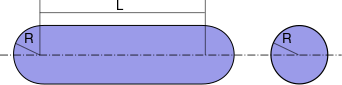
\includegraphics[width=0.7\textwidth]{gota_cilindrica.png}
  \caption{Gota cilíndrica}
  \label{fig:gotaCilindrica}
\end{figure}
